\section{\texorpdfstring{$L^\infty$}{L-infinity}空间}
\label{sec:nspace-linfty-space}

图~\ref{fig:nspace-lp-weight}显示，$p$越大，$L^p$范数越看重大偏差，$p\to\infty$时只剩下最大偏差。向量的情形正是这样：$\lVert v\rVert_p\to\max_i\lvert v_i\rvert$。但等价类中的代表可以在零测集上任意改值，普通的上确界会被单个点左右，对等价类没有确定的意义。本节建立只看“几乎处处”的上界，得到$L^\infty$空间。本节仍固定测度空间$(X,\mathcal A,\mu)$。

\paragraph{本质上确界}
普通上确界要求$\lvert f(x)\rvert\leq M$在每一点都成立；对等价类而言，合理的要求是在某个零测集之外成立。

\begin{definition}[本质上确界与$L^\infty$]
\label{def:nspace-linfty}
对可测函数$f$，定义
\begin{equation}
 \lVert f\rVert_\infty=\inf\{M\geq0:\ \mu(\{x:\lvert f(x)\rvert>M\})=0\},
 \label{eq:nspace-esssup}
\end{equation}
称为$\lvert f\rvert$的\term{本质上确界}（essential supremum），约定空集的下确界为$+\infty$。本质上确界有限的可测函数称为\term{本质有界}（essentially bounded）的，其几乎处处等价类全体记为$L^\infty(\mu)$。
\end{definition}

先看下确界能否取到。设$M_0=\lVert f\rVert_\infty<\infty$。对每个正整数$k$，$M_0+1/k$大于下确界，所以$\{\lvert f\rvert>M_0+1/k\}$是零测集。它们的并
\[
 \{\lvert f\rvert>M_0\}=\bigcup_{k\geq1}\Bigl\{\lvert f\rvert>M_0+\frac1k\Bigr\}
\]
是可数个零测集之并，仍为零测集。所以下确界可以达到：
\begin{equation}
 \lvert f\rvert\leq\lVert f\rVert_\infty\quad\text{几乎处处}.
 \label{eq:nspace-esssup-attained}
\end{equation}
由此也看出数值不依赖代表：若$g\sim_\mu f$，则$\{\lvert g\rvert>M\}\subseteq\{\lvert f\rvert>M\}\cup\{f\neq g\}$，反之亦然，两者的本质上确界相同。

\paragraph{与逐点上确界的比较}
本质上确界与普通上确界可以相差很远。在$[0,1]$上取Lebesgue测度，令$f(x)=x$，再把$f(\tfrac12)$改为$2$。普通上确界是$2$；而$\lvert f\rvert\leq1$只在单点$\{\tfrac12\}$处不成立，单点零测，所以本质上确界是$1$，如图~\ref{fig:nspace-essential-sup}所示。

\begin{BookInlineFigure}
  \centering
  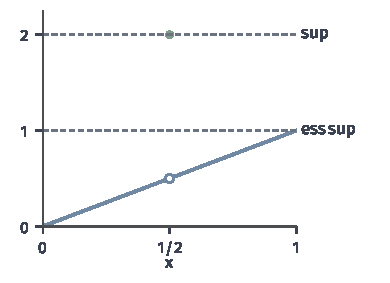
\includegraphics[width=66mm]{figures/04-spaces-measures-and-geometry/03-function-spaces/matplotlib/nspace-essential-sup/figure.pdf}
  \caption{本质上确界忽略零测集。$[0,1]$上取Lebesgue测度，$f(x)=x$，只把$f(\tfrac12)$改为$2$（绿点为改动后的值，空心圈为原值）。普通上确界被这一个点抬到$2$，单点的测度为零，本质上确界仍为$1$。}
  \label{fig:nspace-essential-sup}
\end{BookInlineFigure}

更极端地，有理点的指示函数$\mathbf 1_{\mathbb Q\cap[0,1]}$的普通上确界是$1$，本质上确界是$0$，因为有理点只有可数个，组成零测集。

两者在一个常见情形下一致。若$f$在区间$[a,b]$上连续，对任意$M<\sup\lvert f\rvert$，集合$\{\lvert f\rvert>M\}$是非空的相对开集，含有一个正长度的区间，测度为正，所以本质上确界不小于普通上确界，二者相等。另一方面，$\lVert f\rVert_\infty\leq M$只保证零测集之外$\lvert f\rvert\leq M$，并不保证类中任意一个代表在每一点都受这个界控制。

取$\mathbb N_+$上的计数测度，只有空集零测，本质上确界就是普通上确界，得到有界数列空间
\begin{equation}
 \ell^\infty=\Bigl\{x:\ \sup_{k}\lvert x_k\rvert<\infty\Bigr\},\qquad \lVert x\rVert_\infty=\sup_k\lvert x_k\rvert.
 \label{eq:nspace-ellinfty}
\end{equation}
常数列$(1,1,\ldots)$属于$\ell^\infty$，却不属于任何$\ell^p$（$p<\infty$）。第~\ref{chap:functions-as-vectors}章用$\ell^\infty$中两两距离为$1$的不可数个$0$--$1$数列，说明了它没有可数的级数表示。

\paragraph{范数公理}
$\lVert\cdot\rVert_\infty$在$L^\infty(\mu)$上是范数，论证的关键是把例外集合合并成一个零测集。

正定性：若$\lVert f\rVert_\infty=0$，由式~\eqref{eq:nspace-esssup-attained}，$\lvert f\rvert\leq0$几乎处处，即$[f]$是零元素。齐次性：$c\neq0$时，
\[
 \{\lvert cf\rvert>\lvert c\rvert M\}=\{\lvert f\rvert>M\},
\]
对$M$取下确界即得；$c=0$时两边都是零。

三角不等式：$\lvert f\rvert\leq\lVert f\rVert_\infty$在零测集$N_f$之外成立，$\lvert g\rvert\leq\lVert g\rVert_\infty$在零测集$N_g$之外成立。于是在$N_f\cup N_g$之外，
\[
 \lvert f+g\rvert\leq\lvert f\rvert+\lvert g\rvert\leq\lVert f\rVert_\infty+\lVert g\rVert_\infty.
\]
例外集仍是零测集，所以右边是$\lvert f+g\rvert$的一个本质上界，三角不等式成立。这同时说明$L^\infty(\mu)$对加法封闭。

\paragraph{\texorpdfstring{$L^1$}{L1}与\texorpdfstring{$L^\infty$}{L-infinity}的Hölder估计}
Hölder不等式要求$1<p<\infty$。在端点处，$p=1$的共轭指数应当是$q=\infty$，相应的估计是：若$f\in L^1(\mu)$、$g\in L^\infty(\mu)$，则
\begin{equation}
 \int_X\lvert fg\rvert\,d\mu\leq\lVert f\rVert_1\,\lVert g\rVert_\infty .
 \label{eq:nspace-holder-endpoint}
\end{equation}

证明只需一步。由式~\eqref{eq:nspace-esssup-attained}，几乎处处有
\[
 \lvert fg\rvert\leq\lvert f\rvert\,\lVert g\rVert_\infty,
\]
两边积分即可。约定$1/\infty=0$后，Hölder不等式对所有满足$\tfrac1p+\tfrac1q=1$的$1\leq p,q\leq\infty$都成立。

这个估计说明，固定$g\in L^\infty$，$f\mapsto\int fg\,d\mu$是$L^1$上的线性读取，其大小受$\lVert g\rVert_\infty\lVert f\rVert_1$控制。第~\ref{chap:linear-functionals}章将从这样的配对出发研究$L^p$上的线性泛函。

\paragraph{完备性}
$L^\infty$的完备性与$L^p$（$p<\infty$）的证明方式不同。这里没有积分可以累计，却可以把可数个例外集合并成一个零测集，在它的补集上回到一致收敛的论证。

\begin{theorem}[$L^\infty$的完备性]
\label{thm:nspace-linfty-complete}
对任意测度空间，$L^\infty(\mu)$是Banach空间。
\end{theorem}

\begin{proof}
设$(f_n)$是$L^\infty(\mu)$中的柯西列，取定各项的可测代表。对每一对$m,n$，由式~\eqref{eq:nspace-esssup-attained}，在某个零测集$E_{m,n}$之外有
\[
 \lvert f_n-f_m\rvert\leq\lVert f_n-f_m\rVert_\infty.
\]
令$E=\bigcup_{m,n}E_{m,n}$，它是可数个零测集之并，仍为零测集。

在$X\setminus E$上，所有这些不等式同时成立。给定$\varepsilon>0$，取$N$使$m,n\geq N$时$\lVert f_n-f_m\rVert_\infty<\varepsilon$，则
\[
 \sup_{x\notin E}\lvert f_n(x)-f_m(x)\rvert\leq\varepsilon,\qquad m,n\geq N,
\]
即$(f_n)$在$X\setminus E$上一致柯西。$\mathbb K$完备，所以$f_n$在$X\setminus E$上一致收敛到某个函数$f$；在$E$上令$f=0$。$f$是可测函数列在$X\setminus E$上的逐点极限，因而可测。

在上式中令$m\to\infty$，得到$n\geq N$时
\[
 \sup_{x\notin E}\lvert f_n(x)-f(x)\rvert\leq\varepsilon.
\]
$E$零测，所以$\lVert f_n-f\rVert_\infty\leq\varepsilon$，即$f_n\to f$依范数成立。最后，取$n_0\geq N$，由三角不等式，
\[
 \lVert f\rVert_\infty\leq\lVert f_{n_0}\rVert_\infty+\varepsilon<\infty,
\]
所以$f\in L^\infty(\mu)$。
\end{proof}

两种完备性证明可以对照着看。有限$p$的论证没有一致性可用，只能先抽子列得到几乎处处收敛，再用Fatou引理把逐点信息转为积分信息。$p=\infty$的论证则把可数个例外集合并成一个零测集，在补集上做一致收敛，与连续函数空间的论证相同，只是“处处”换成了“零测集之外”。

在计数测度下，这个定理说明$\ell^\infty$是Banach空间。
